\documentclass[ukrainian,14pt]{extarticle}
%\documentclass[14pt]{


\usepackage[T1]{fontenc}
\usepackage{lmodern}
\usepackage{babel}
\usepackage[utf8]{inputenc}
\usepackage{fullpage}
\usepackage{ upgreek }
\usepackage{amsmath}
\usepackage{pifont}
\usepackage[bookmarks=true]{hyperref}
\usepackage{bookmark}
\usepackage{graphicx}
\usepackage{tocloft}
\usepackage{listings}
\usepackage{indentfirst}

\usepackage{listings}
\usepackage{color}
 
\definecolor{codegreen}{rgb}{0,0.6,0}
\definecolor{codegray}{rgb}{0.5,0.5,0.5}
\definecolor{codepurple}{rgb}{0.58,0,0.82}
\definecolor{backcolour}{rgb}{0.95,0.95,0.92}
 
\lstdefinestyle{mystyle}{
    backgroundcolor=\color{backcolour},   
    commentstyle=\color{codegreen},
    keywordstyle=\color{magenta},
    numberstyle=\tiny\color{codegray},
    stringstyle=\color{codepurple},
    basicstyle=\footnotesize,
    breakatwhitespace=false,         
    breaklines=true,                 
    captionpos=b,                    
    keepspaces=true,                 
    numbers=left,                    
    numbersep=5pt,                  
    showspaces=false,                
    showstringspaces=false,
    showtabs=false,                  
    tabsize=2
}
 
\lstset{style=mystyle}




\renewcommand\cftsecleader{\cftdotfill{\cftdotsep}}

\def\ab{[a,b]}
\newcommand{\sign}{\operatorname{sign}}

\begin{document}

\title{
	Звіт \\
	про проходження практики за темою \\
	бакалаврської кваліфікаційної роботи\\
    "Моделювання функціональних залежностей \\
	мінімаксними многочленними наближеннями"
}
\author{ст. гр. ПМ-41 \\  Левантович Богдан}

\makeatletter
\begin{titlepage}
        \centering
	МІНІСТЕРСТВО ОСВІТИ І НАУКИ УКРАЇНИ \\
	НАЦІОНАЛЬНИЙ УНІВЕРСИТЕТ "ЛЬВІВСЬКА ПОЛІТЕХНІКА" \\
	Інститут прикладної математики та фундаментальних наук\\
	\vspace{20pt}
	
	\begin{flushright}
	Кафедра прикладної математики
	\end{flushright}
	\vspace{30pt}
	\centering
	\vspace{\fill}

	\@title \\
	\vspace{100pt}
	\raggedright
        \setlength{\leftskip}{11cm}
	Виконав:\\
	\@author\\
        Керівник БКР:\\
        доц. каф. ПМ \\
        Пізюр Я.В.\\
	Прийняв: \\
	Гладун В.Р. керівник \\
	практики від університету\\
        \setlength{\leftskip}{0cm}
	\vspace{80pt}
	\centering


	Львів 2017
\end{titlepage}
\makeatother

\setcounter{page}{2}
\tableofcontents

\newpage


\section*{Вступ}
\addcontentsline{toc}{section}{Вступ}

%Далі розглянемо властивості найкращих наближень многочленом. 

%\addcontentsline{toc}{section}{Вступ}
Необхідність моделювання функціональних залежностей виникає в багатьох галузях прикладної математики та інформатики. При розв’язуваннi багатьох задач науково-технiчного характеру доводиться використовувати функції задані таблицею. Проте часто необхідно мати значення функції в точках, яких немає в таблиці. Також виникає необхідність використання простої функції замість складної. 


Багатьом із тих, хто стикається з науковими та інженерними розрахунками часто доводиться оперувати наборами значень, отриманих експериментальним шляхом чи методом випадкової вибірки. Як правило, на підставі цих наборів потрібно побудувати функцію, зі значеннями якої могли б з високою точністю збігатися інші отримувані значення. Така задача називається апроксимацією кривої. Інтерполяцією називають такий різновид апроксимації, при якій крива побудованої функції проходить точно через наявні точки даних.

\newpage


\section{Найкраще чебишовське наближення}
%\addcontentsline{toc}{section}{Найкраще чебишовське наближення}

За теоремою Вейєрштрасса для довільних неперервних на обмеженому проміжку $[a,b]$   
функцій $f(x)$ та $w(x) > 0$ і довільного $\epsilon > 0$ можна знайти такий многочлен $P_m(x)$, що

$$|\rho(x)| = \frac{|f(x) - P_m(x)|}{w(x)} < \epsilon, \quad x \in [a,b].$$

Ясно, що найменше при цьому значення степеня $m$ многочлена $P_m(x)$ суттєво залежить від способу наближення. Серед усіх способів наближення функцій найменшу похибку a, значить, і найменше $m$ при заданому $\epsilon$, дає найкраще чебишовське наближення.

Вираз $F(A,x) \in F(B,x)$, для якого максимальне значення абсолютної величини зваженої похибки досягає на проміжку $[a,b]$ найменшого значення

\begin{equation}\label{eq:formula4}
\min_{c \in B} \max_{x \in [a,b]} \frac{|f(x) - F(C,x)|}{w(x)} = \max_{x \in [a,b]} \frac{|f(x) - F(A,x)|}{w(x)},
\end{equation}
звемо найкращим чебишовським зваженим (з вагою $w(x)$) наближенням функції $f(x)$ за допомогою виразу виду $F(A,x)$ на проміжку $[a,b]$.

У цій курсові розглянуто лише найкращі чебишовські наближення. Слова ``чебишовські'' і ``зважені'' будемо часом пропускати. При $w(x) = 1$ маємо найкраще абсолютне наближення, при $w(x) = f(x)$ - найкраще відносне.

Величину (\ref{eq:formula4}) називатимемо мінімальним (зваженим) відхиленням і позначаємо $E(f,W)\equiv\mu_0$; $E(f,1) \equiv E(f) \equiv \Delta_0$ - мінімальне абсолютне відхилення; $E(f,f) \equiv \delta_0$ - мінімальне відносне відхилення.

Далі розглянемо властивості найкращих наближень многочленом.\\

\noindent
\textbf{Теорема 1.}\textit{
Для будь-яких неперервних на проміжку $[a,b]$ функцій $f(x)$ та $w(x) > 0$ і довільного $\epsilon$, існує єдиний многочлен $P_m(x)$ степеня $m$, що має найменше відхилення $E(f,w)$.}\\

\noindent
\textbf{Теорема 2.}\textit{
Нехай на проміжку $[a,b]$ задано неперервні функції $f(x)$ та $w(x) > 0$.
Тоді для того, щоб деякий многочлен $P_m(x)$ степеня не вище $m$ був многочленом найкращого чебишовського зваженого наближення функції $f(x)$ на проміжку $\ab$ необхідно і достатньо, щоб на цьому проміжку знайшлась принаймні одна система з $m+2$ точок \\ $T=\{t_k\}_{k=0}^{m+1} \quad a \leq t_0 < t_1 < t_2 < \ldots \leq t_{m+1}$, у яких зважена різниця  почергово набувала значень різних знаків і досягала за модулем найбільшого на $\ab$ значення тобто:
}
\begin{equation}\label{eq:formula5}
\rho(t_0) = -\rho(t_1) = \rho(t_2) = \ldots = (-1)^{m+1}\rho(t_{m+1}) = \pm E(f,W).
\end{equation}\\


Система точок $T$ із теореми 2 зветься системою точок (чебишовського альтернансу). Для побудови многочлена найкращого наближення  необхідно визначити ці точки. Точно визначити їх значення можна тільки у часткових випадках. 

\subsection{Cхема Ремеза побудови чебишовського наближення}
%\addcontentsline{toc}{subsection}{Cхема Ремеза побудови чебишоського наближення}

У загальному випадку процес знаходження точок $T$ побудовано на ітераційних методах. Найбільше практичне значення мають методи розроблені українським математиком Є.Я. Ремезом. Коротко розглянемо один з методів. Він складається з таких етапів.

\begin{enumerate}
	\item З проміжку $\ab$ вибираємо початкове наближення $T_0$ до альтернансу
	$$T: t^{(0)}_{0} < t^{(0)}_{1} < t^{(0)}_{2} < \ldots < t^{(0)}_{m+1}.$$
	Можна, наприклад, прийняти $t^{(0)}_k = a + \frac{(b-a)k}{m+1}$.
	
	\item Здійснюємо чебишовську інтерполяцію для множини точок  \\ $T_j = \{t_k\}_{k=0}^{m+1}, t^{(j)}_k < t^{(j)}_{k+1}, k=\overline{0,m}$, тобто визначаємо коефіцієнти многочлена $P^{i}_m(x)$ і величину $\mu_j$, для яких виконуються умови $\rho(t^{(j)}_k) = (-1)^{k} \mu_k \quad k = \overline{0, m+1}$. Для знаходження вказаних величин розв'язуємо систему рівнянь:

\begin{equation}\label{eq:formula6}
\begin{cases}
f(t^{(j)}_0) - a_0 - a_1t^{(j)}_0 - \ldots - a_m(t_0^{(j)})^m=\mu_jw(t_0^{(j)}), \\
f(t^{(j)}_1)-a_0-a_1t^{(j)}_1 - \ldots - a_m(t^{(j)}_1)^m = - \mu_jw(t^{(j)}_1),\\
\dotfill\hfill\hbox{} \dotfill\hfill\hbox{}\\
f(t^{(j)}_{m+1}) -a_0 -a_1t^{(j)}_{m+1} - \ldots - a_m(t^{(j)}_{m+1})^m = (-1)^{m+1}\mu_jw(t^{(j)}_{m+1}).
\end{cases}
\end{equation}
$$$$
Система є системою $m+2$ алгебраїчних рівнянь з $m+2$ невідомими: $a_0, a_1, \ldots ,a_m$ та $\mu$.

\item Перевіряємо виконання рівності
\
\begin{equation}\label{eq:formula7}
|\mu_j| = \max_{x \in [a,b]} |f(x) - P^{(j)}_m(x)| / w(x) \equiv \rho_j.
\end{equation}

Якщо рівність виконується, то у відповідності з теоремою 2 многочлен $P^{(j)}_m(x)$ і є шуканий многочлен найкращого наближення. При машинній реалізації алгоритму перевірку рівності заміняють перевіркою нерівності

\begin{equation}\label{eq:formula8}
\rho_j - |\mu_j|\leq \epsilon|\mu_j|,
\end{equation}
де $\epsilon$ - допустима відносна помилка у визначенні похибки наближення. Можна, наприклад, прийняти $\epsilon = 10^{-2}$ чи $\epsilon = 10^{-3}$.
\item
Якщо умова \ref{eq:formula7} чи \ref{eq:formula8} не виконується, то приймаємо $j:=j+1$ і вибираємо наступне (уточнене) наближення до точок чебишовського альтернансу (наступний V-альтернанс). Далі виконання алгоритму повторюється починаючи з п.2.

При обчисленнях на ЕОМ у цьому пункті іноді додатково перевіряються умови
$$\left|t^{(j-1)}_k - t^{j}_k\right| < \eta, \quad k = \overline{0, m+1},$$

де $\eta$ - допустима помилка у визначенні точок альтернансу. Якщо остання нерівність справедлива для всіх точок $k = \overline{0, m+1}$, то вважаємо, що многочлен найкращого наближення знайдено.

\end{enumerate}
\subsection{Алгоритм Валле-Пуссена заміни точок альтернансу}
%\addcontentsline{toc}{subsection}{Алгоритм Валле-Пуссена заміни точок альтернансу}

Існує кілька методів заміни точок альтернансу. Можлива заміна одної або кількох точок одночасно. Найпростішим алгоритмом є алгоритм Є.Я. Ремеза з одноточковою заміною (алгоритм Валлє-Пуссена). Опишемо цей алгоритм.

Нехай при виконанні п.3 знайдена точка $\tilde{x}$, для якої справедливо $\rho_j = |\rho(\tilde{x})|$. Можливі три випадки взаємного розміщення точок V-альтернансу та точки $\tilde{x}$:
	\begin{enumerate}
		\item[1.] $t^{(j)}_0 < \tilde{x} < t^{(j)}_{m+1} $
		\item[2.] $\tilde{x} < t^{(j)}_{0}$
		\item[3.] $\tilde{x} > t^{(j)}_{m+1}$
	\end{enumerate}
	
	Розглянемо спосіб заміни точок V-альтернансу у кожному випадку.
	
	\begin{enumerate}
	\item Знайдемо ціле число $v$ таке, що $t^{(j)}_v < \tilde{x} < t^{(j)}_{v+1}$. Якщо $\sign(\rho(\tilde{x})) = \sign(\rho(t^{(j)}_{m+1}))$, то приймаємо $t^{(j+1)}_v := \tilde{x}$, у протилежному випадку $t^{(j+1)}_{v+1}:=\tilde{x}$. Решту точок V-альтеранансу не змінюємо.
	\item Якщо $\sign \rho(\tilde{x}) = \sign \rho(t^{(j)}_0)$, то приймаємо $t^{(j+1)}_0 := \tilde{x}$, а решту точок V-альтернансу не змінюємо. Якщо це не так, то заміняємо усі точки альтернансу за формулами:
	$$t^{(j+1)}_{0}:=\tilde{x};\quad t^{(j+1)}_k := t^{(j)}_{k-1}, \quad k=\overline{1, m+1}.$$
	У цьому випадку із V-альтернансу виключається точка $t^{(j)}_{m+1}$
	
	\item Якщо $\sign \rho(\tilde{x}) = \sign \rho(t^{(j)}_{m+1})$, то приймаємо $t^{(j)}_{m+1}:=\tilde{x}.$ і решту точок V-альтернансу не змінюємо. Якщо це не так, то замінюємо усі точки V-альтернансу за формулами:
	$$t^{(j+1)}_k := t^{(j)}_{k+1}, \quad k=\overline{0,m}; \quad t^{(j+1)}_{m+1}:=\tilde{x}.$$
	У цьому випадку із V-альтернансу виключається точка $t^{(j)}_0$.
	\end{enumerate}
	Отже черговий V-альтернанс відрізняєтся від попереднього тим, що точка $\tilde{x}$, у якій досягається максимум абсолютної величини зваженої похибки, вводиться у V-альтернанс замість однієї із старих точок.
	Відомо, що алгоритм Валле-Пуссена для заміни точок альтернансу при знаходженні найкращого наближення попередньої функції многочленом на проміжку $[a,b]$ збігається незалежно від початкового наближення до точок альтернансу. Більш того у цьому випадку цей алгоритм збігається зі швидкістю гометричної прогресії у тому сенсі, що знайдуться такі числа $A$ та $0 < q < 1$, що відхилення $E^{(k)}(f,W)$ многочлена $P^{(k)}_m(x)$ від функції $f(x)$ будуть задовольняти нерівності
	$$E^{(k)}(f,W) - E(f,W) \leq Aq^k; \quad k=1,2,\ldots$$
Фактична швидкість збіжності залежить від диференціальних властивостей функції та використовуваного алгоритму	 заміни точок альтернансу. Відомо, що коли $f(x) \in C^{m+1} [a,b], w(x) = 1$ або $w(x) = f(x)$ і $f^{(m+1)}(x)$ не змінює знак при $x \in [a,b]$, то граничні точки проміжку $[a,b]$ є точками альтернансу. Тому у цьому випадку алгоритм Валле-Пуссена для наближення многочленами невисоких степенів $m = \overline{0, 2}$ практично не програє у швидкості порівняно з іншими алгоритмами типу Є.Я. Ремеза.
Зазначимо, що всі перелічені властивості найкращого чебишовського наближення непервної при $x \in [a,b]$ функції $f(x)$ многочленом справедливі також і для наближення табличної функції. Більш того, при заміні неперервної функції її значенями в точках $x_k = a + \frac{(b-a)k}{N}$ різниця між відповідними відхиленнями при $N\rightarrow\infty$ прямує до нуля.

\newpage

\subsection{Опис програми}
%\addcontentsline{toc}{section}{Опис програми}

Мета програми: знаходження найкращого чебишовського наближення для заданої функції. \\
Програма написана на мові програмування \emph{Python} з використанням таких бібліотек: \emph{Sympy, Numpy, Plotly}.
\subsubsection{Вхідні дані}
%\addcontentsline{toc}{subsection}{Вхідні дані}

\begin{enumerate}
\item Початок інтервалу.
\item Кінець інтервалу.
\item Степінь многочлена.
\item Функція для апроксимації.
\item Точність (за замовчуванням $10^{-2}$).
\end{enumerate}

\subsubsection{Вихідні дані}
%\addcontentsline{toc}{subsection}{Вихідні дані}

\begin{enumerate}
\item Коефіцієнти многочлена.
\item Графіки похибок на кожній ітерації.
\item Графік многочлена і функції.

\end{enumerate}
\newpage

\section{Метод найменших квадратiв}
\subsection{Опис алгоритму}
Нехай в результатi вимiрювань величини, яка описується функцiєю
$y(x)$ при $x = x_1, x = x_2, \ldots , x = x_n, x_i \in [a, b], \quad i = \overline{1,n}$ отримаємо таблицю значень $y_i, i = \overline{1, n}$. За даними таблицi треба побудувати аналiтичну
формулу

% add label
\begin{equation}\label{eq:formula9}
    \overline{y}(x) = f(x, a_1, \ldots , a_m),
\end{equation}
яка залежить вiд $m \quad(m < n)$ параметрiв $a_i, i = \overline{1, m}$, причому функцiя
$\overline{y}(x)$ має "досить добре"    наближувати функцiю $y(x)$ на всьому промiжку
$[a, b]$. Вигляд функцiї $f$ i кiлькiсть параметрiв у деяких випадках
вiдомi на основi додаткових мiркувань. В iнших випадках вони визначаються за графiком,
 побудованим за вiдомими значеннями $y(x_i)$ так,
щоб залежнiсть (\ref{eq:formula9}) була досить простою i добре вiдображала результати спостережень.
Якщо система рiвнянь

\begin{equation}\label{eq:formula10}
\begin{cases}
    y_1 = f(x_1, a_1, \ldots , a_m), \\
	\ldots \ldots \ldots \ldots  \ldots \ldots \ldots\\
y_n = f(x_n, a_1, \ldots , a_m)
\end{cases}
\end{equation}

має єдиний розв’язок, то вiн може бути знайдений з яких-небудь m рiв-
нянь системи (\ref{eq:formula10}). Однак, у загальному випадку значення $yi, xi, i = \overline{1, n}$
є наближеними i точний вигляд залежностi $\overline{y}(x)$ невiдомий i через
це система (\ref{eq:formula10}) переважно є несумiсною. Тому визначимо параметри
$a_1, \ldots , a_m $ так, щоб у деякому розумiннi всi рiвняння системи (\ref{eq:formula10}) задовольнялися
 з найменшою похибкою, точнiше, щоб мiнiмiзувати функцiю
$$
 S(a_1, \ldots , a_m) = \sum_{i=1}^n [y_i - f (x_i, a_1, \ldots , a_m)]^2.
$$
Такий метод розв'язання системи (\ref{eq:formula10}) називається методом найменших квадратiв.
Якщо функцiя  $S(a_1, \ldots , a_m)$ досягає абсолютного мiнiмуму в областi змiни 
параметрiв $a_1, \ldots , a_m$, то, розв'язуючи систему

$$
    \frac{\partial S}{\partial a_k} = -2 \sum_{i=1}^n [y_i - f(x, a_1, \ldots , a_m)] 
     \frac{\partial f(x, a_1, \ldots , a_m)}{\partial a_k}, \quad k = \overline{1,m},
$$

знаходимо точки, в яких може бути екстремум. Вибравши той розв'язок, 
який належить областi змiни параметрiв $a_1, \ldots , a_m$ i в якому функцiя
$S(a_1, \ldots , a_m)$ має абсолютний мiнiмум, знаходимо незалежнi значення
 $a_1, \ldots , a_m$
Якщо $f(x, a_1, \ldots , a_m)$ лiнiйно залежить вiд параметрiв $a_1, \ldots , a_m$, тобто

$$ f(x, a_1, \ldots , a_m) = \sum_{j=1}^m f_j(x)a_j,$$
то система (\ref{eq:formula10}) набуває вигляду
\begin{equation}\label{eq:formula11}
    y_i = \sum_{j=1}^m f_j(x)a_j, \quad i = \overline{1,n}.
\end{equation}

Метод найменших квадратiв розв'язування системи (\ref{eq:formula11}) полягає у
тому, щоб визначити невiдомi, якi мiнiмiзують суму квадратiв нев'язок,
тобто суму вигляду

$$ S(a_1, \ldots , a_m) = \sum_{i=1}^n  \left[y_i - \sum_{j=1}^m f_j(x)a_j \right]^2.	$$

З умови мiнiмуму величини $S$ як функцiї вiд $a_1, \ldots , a_m$ отримаємо систему
лiнiйних алгебраїчних рiвнянь

$$\frac{\partial S}{\partial a_k} = -2 \sum_{i=1}^n \left[y_i - \sum_{j=1}^m f_j(x)a_j \right] f_k(x_i) = 0, \quad k=\overline{1,m},$$
або
$$\sum_{i=1}^n \left[\sum_{j=1}^m f_j(x_i)a_j \right]f_k(x_i) = \sum_{i=1}^n f_k(x_i)y_i, \quad k=\overline{1,m}.$$
Розв'язок системи $m$ лiнiйних алгебраїчних рiвнянь з $m$ невiдомими вважаємо наближеним розв’язком системи.

\newpage

\subsection{Опис програми}
Програму для пошуку апроксимації для функції методом найменших квадратів я написав на мові \textit{Python}. Також зробив web сайт
який можна переглянути за адресою
\href{http://least-squares.herokuapp.com/}{http://least-squares.herokuapp.com/}. 

\subsubsection{Вхідні дані}

Користувачу пропонується ввести функцію яку він хоче апроксимувати методом найменших квадратів. Також степінь многочлена, інтервал на якому апроксимується функція, кількість точок які будуть використовуватися в методі найменших квадратів і кількість цифр після коми.

\subsubsection{Вихідні дані}

Після того як користувач натисне кнопку «Знайти», на екрані браузера появиться вигляд многочлена, максимальна похибка, та значення $x$ в якому ця похибка досягається.
\newpage

\section*{Висновки}
\addcontentsline{toc}{section}{Висновки}
У цій роботі я розглянув найкраще чебишовське наближення многочленами. Написав програму для знаходження коефіцієнтів такого многочлена. Також в програмі реалізув побудову графіків похибок на кожній ітерації, вивід максимальної похибки та значення аргументу при якому ця похибка досягається.

Також розглянув метод найменших квадратів. Написав програму яка реалізує алгоритм МНК на мові \textit{Python}. Зробив web сайт для зручного пошуку апроксимації для функції.
%Розглянуто основні поняття наближення функцій та рівномірного наближення функцій сплайнами. Введено поняття найкращого чебишовського наближення та розглянуті властивості такого наближення многочленами. Розглянуто етапи знаходження коефіцієнтів найкращого чебишовського многочленного наближення. Для многочленів невеликих степенів виведено формули для коефіцієнтів. Виведена загальна формула для похибки рівномірного наближення аналітичних функцій сплайнами. Розглянуто її частинні випадки для многочленних сплайнів. Досліджено частинні випадки: рівномірне наближення відрізками сталих та рівномірне наближення сталою.

\newpage

\section*{Список використаної літератури}
\addcontentsline{toc}{section}{Список використаної літератури}

\begin{enumerate}
\item  Демьянов В.Ф., Малоземов В.Н. Введение в минимакс. -М.: Наука, 1972. - 368 с.
\item Попов Б.А. Равномерное приближение сплайнами. -Киев: Наук. думка, 1989. - 272 с.
\item Попов Б.А., Теслер Г.С. Приближение функций для технических приложений. - Киев: Наук. думка, 1980. - 352 с.
\item Ремез Е.Я. Основы численных методов чебышовского приближения. Киев: Наук. думка, 1969, - 623 с.
\item Попов Б.О. Чисельні методи рівномірного наближення сплайнами. Конспект лекцій. -Львів: ЛДУ, 1992. - 92 с.
\item Самарский А.А., Гулин А.В. Численные методы. -М.: Наука, 1989. - 432 с.
\item Самарский А.А., Гулин А.В. Численные методы. -М.: Наука, 1989. - 432 с.
\item Кутнів М.В. Чисельнi методи: Навчальний посiбник.— Львiв, 2010. –286 с.

\item https://plot.ly/ - для побудови графіків
\item http://www.sympy.org/ - для розв'язування систем
\item http://www.numpy.org/ - для наукових розрахунків
\end{enumerate}

\newpage

\section{Додатки}


\subsection{Приклади виконання програми(чебишовське наближення)}
\textbf{Приклад 1} 	
%\addcontentsline{toc}{section}{Приклади виконання програми}

Знайдемо чебишовське наближення поліномом степеня 2 для функції $f(x) = ln(x)$ на проміжку $[1, 4]$. Точність ($\epsilon = 0.01$)

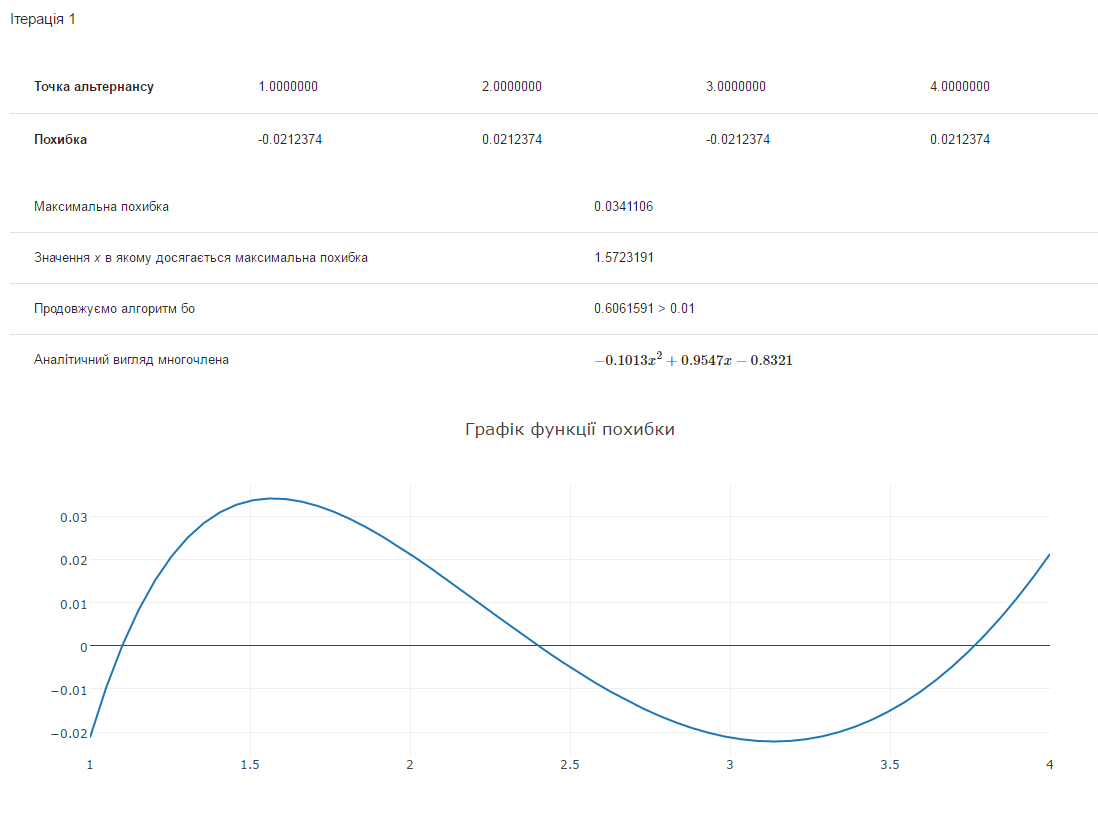
\includegraphics[scale=0.6]{exp_err_1}
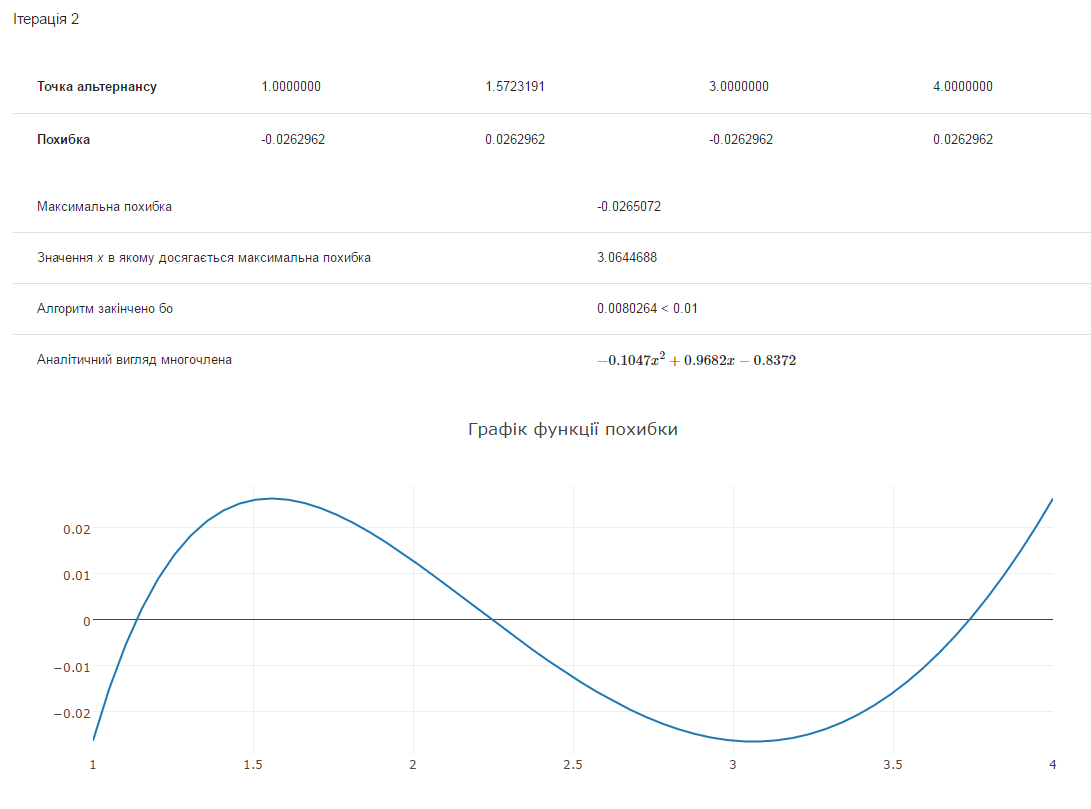
\includegraphics[scale=0.6]{exp_err_2}

Перевіримо умову завершення алгоритму: $\frac{\rho_j - |\mu_j|}{|\mu_j|} \leq \epsilon.$ \\

$$\frac{0.0265072 - 0.0262962}{0.0262962} \approx 0.00802 < \epsilon = 0.01$$
Оскільки умова виконується  то многочлен чебишовського наближення знайдено. Його вигляд:\\
$$P_2(x) = -0.10474 x^{2} + 0.96826x - 0.83723$$


\newpage
\subsection{Приклади виконання програми (МНК)}
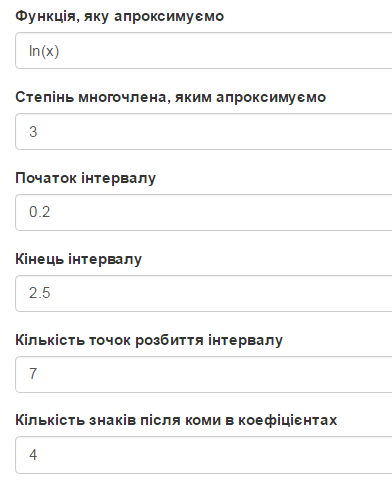
\includegraphics[scale=0.7]{form} \\
Результати роботи програми \\
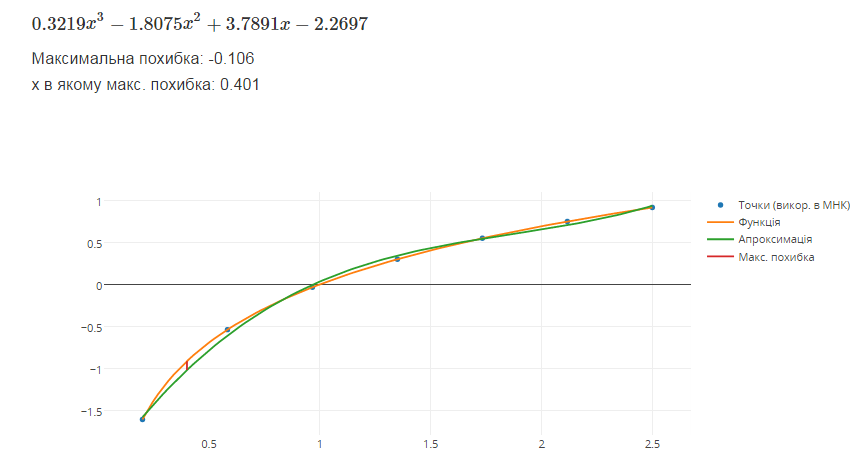
\includegraphics[scale=0.7]{res}

\end{document}